%%%%%%%%%%%%%%%%%%%%%%%%%%%%%%%%%%%%%%%%%%%%%%%%%%%%%%%%%%%%%%%
%
% Welcome to Overleaf --- just edit your LaTeX on the left,
% and we'll compile it for you on the right. If you open the
% 'Share' menu, you can invite other users to edit at the same
% time. See www.overleaf.com/learn for more info. Enjoy!
%
%%%%%%%%%%%%%%%%%%%%%%%%%%%%%%%%%%%%%%%%%%%%%%%%%%%%%%%%%%%%%%%
% --------------------------------------------------------------
% This is all preamble stuff that you don't have to worry about.
% Head down to where it says "Start here"
% --------------------------------------------------------------
 
\documentclass[12pt]{article}
 
\usepackage[margin=1in]{geometry} 
\usepackage{amsmath,amsthm,amssymb}
\usepackage{graphicx}
\usepackage{enumitem}
\usepackage{xcolor}
\definecolor{smithblue}{HTML}{002855}
\definecolor{smithyellow}{HTML}{F2A900}
\usepackage{textcomp}
\usepackage{enumitem}
\usepackage{tkz-berge}

\usepackage[parfill]{parskip}
\parskip=\baselineskip
 
\newcommand{\N}{\mathbb{N}}
\newcommand{\Z}{\mathbb{Z}}
 
\newenvironment{theorem}[2][Theorem]{\begin{trivlist}
\item[\hskip \labelsep {\bfseries #1}\hskip \labelsep {\bfseries #2.}]}{\end{trivlist}}
\newenvironment{lemma}[2][Lemma]{\begin{trivlist}
\item[\hskip \labelsep {\bfseries #1}\hskip \labelsep {\bfseries #2.}]}{\end{trivlist}}
\newenvironment{exercise}[2][Exercise]{\begin{trivlist}
\item[\hskip \labelsep {\bfseries #1}\hskip \labelsep {\bfseries #2.}]}{\end{trivlist}}
\newenvironment{reflection}[2][Reflection]{\begin{trivlist}
\item[\hskip \labelsep {\bfseries #1}\hskip \labelsep {\bfseries #2.}]}{\end{trivlist}}
\newenvironment{proposition}[2][Proposition]{\begin{trivlist}
\item[\hskip \labelsep {\bfseries #1}\hskip \labelsep {\bfseries #2.}]}{\end{trivlist}}
\newenvironment{solution}[1][Solution]{\begin{trivlist}
\item[\hskip \labelsep {\bfseries #1}\hskip \labelsep {\bfseries}]}{\end{trivlist}}
\newcommand{\angles}[1]{\textlangle{}$#1$\textrangle{}}

\usepackage{fancyhdr}
\pagestyle{fancy}
\lhead{Submitted by: \studentName\\
\collaborators}
\rhead{CSC250 Fall 2024 - Homework 08\\
\today{}}
\cfoot{p. \thepage}
\renewcommand{\headrulewidth}{0.4pt}
\renewcommand{\footrulewidth}{0.4pt}

% --------------------------------------------------------------
% This is all preamble stuff that you don't have to worry about.
% Head down to where it says "Start here"
% --------------------------------------------------------------

\begin{document}
 
% --------------------------------------------------------------
%                         Start here
% --------------------------------------------------------------


\newcommand{\studentName}{YOUR NAME HERE} %replace with your name

\newcommand{\collaborators}{
	% Comment out the line below if you worked alone
	with \textit{COLLABORATORS' NAMES HERE}
	% Uncomment the line below if you worked alone
	% \textit{I did not collaborate with anyone on this assignment.}
}

\newcommand\answerkey[1]{\vskip 5pt \noindent{\color{red}{\bf Solution:}} \emph{#1}}
 


% \textit{\textbf{Note:} by the end of this assignment, we will have constructed the following chain of $NP$-complete problems:}
% \[SAT \leq_p 3SAT \leq_p CLIQUE \leq_p INDEPENDENT-SET \leq_p VERTEX-COVER\]

% \hrule
% \vskip 2em 
% --------------
% Exercise 1
% --------------
\begin{exercise}{1}
Show that the following language is in $P$:
\[\texttt{RELATIVELY-PRIME}=\{ \langle x,y \rangle \ | \ x \texttt{ and } y \texttt{ are integers, } gcd(x, y) = 1\}\]
\end{exercise}


\hrule
\vskip 1em 

% --------------
% Exercise 2
% --------------
\begin{exercise}{2}
A Caesar cipher is a simplified encryption protocol in which all letters are shifted $0 < k < 26$ positions $mod \ 26$, e.g. when $k=3$:\\\\
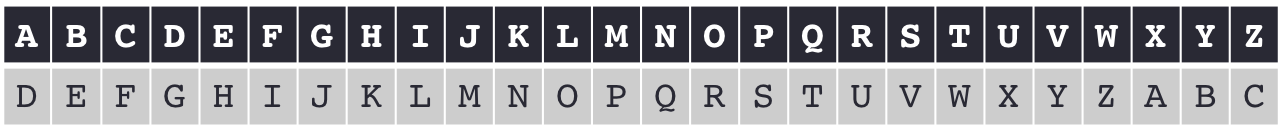
\includegraphics[width=\textwidth]{caesar.png}\\
To use this encryption method, look up the substitution for each letter, like this:
\begin{center}
{\Large SMITH COLLEGE$\rightarrow$ VPLWK FROOHJH}
\end{center}
Show that this encryption scheme can be broken in $O(n)$ where $n$ is the length of the message.
\end{exercise}

%\clearpage
\vskip 1em 
\hrule
\vskip 1em 

% --------------
% Exercise 3
% --------------
\begin{exercise}{3}
Consider the language: 
\begin{eqnarray*}
VERTEX-COVER &=& \{\langle G,k \rangle  \ | \ G \texttt{ is a graph that has a} \\
&&\texttt{ \ \ \ \ \ \ \ vertex cover of size }k\}
\end{eqnarray*}
where a \textbf{vertex cover} is a set of $k$ vertices such that every edge in the graph touches at least one of the vertices.
\begin{enumerate}[label=(\alph*)]
	\item Draw a diagram of a graph on 10 vertices with an \textbf{vertex cover} of size 5.
	\item Prove that $VERTEX-COVER$ is $NP$-complete.
\end{enumerate}
\end{exercise}

\vskip 1em 
\hrule
\vskip 1em 

% --------------
% Exercise 4
% --------------
\begin{exercise}{4}
Consider the language: 
\begin{eqnarray*}
SET-COVER &=& \{\langle U,S,k \rangle  \ | \ U \texttt{ is a set of elements } \{1, 2, ..., n\} \texttt{ (the "universe"),} \\
&& \ \ \ \ \ \ \ \ \ \ \ \ \ \ \ S \texttt{ is a set of } m \texttt{ subsets where } \bigcup S = U, \\
&& \ \ \ \ \ \ \ \ \ \ \ \ \ \ \ \texttt{and } S \texttt{ contains a set cover of size } k\}
\end{eqnarray*}
where a \textbf{set cover} is a set of $k$ subsets $\in S$ such that every element in $U$ is contained in at least one of the selected subsets.\\

\begin{enumerate}[label=(\alph*)]
	\item Draw a diagram of a universe with 10 elements, partitioned into 5 subsets with a \textbf{set cover} of size 3.
	\item Prove that $SET-COVER$ is $NP$-complete.
\end{enumerate}
\end{exercise}


% ------------------------------------------------------------------
%     DON'T FORGET TO INCLUDE REFERENCES
% ------------------------------------------------------------------
\section*{References}

% --------------------------------------------------------------
%     You don't have to mess with anything below this line.
% --------------------------------------------------------------
 
\end{document}